\newpage
\begin{figure}[h]
	\centering
	\caption{UCA 7 - Visualizzazione storico accessi presso un’organizzazione}
	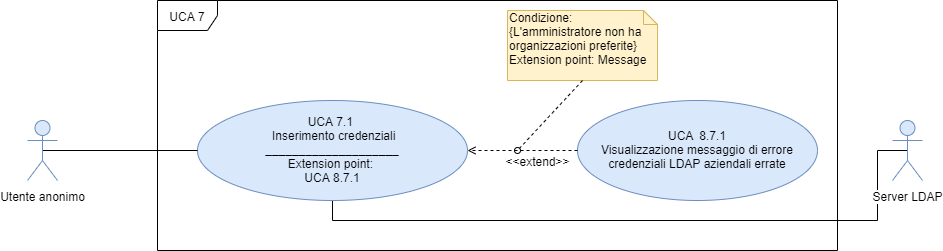
\includegraphics[scale=0.5]{sezioni/UseCase/Immagini/UCA7.png}
\end{figure}
\section{UCA 7 Visualizzazione storico accessi presso un’organizzazione}%kite level
\begin{itemize}
\item \textbf{Attori primari:} Utente anonimo;
\item \textbf{Precondizione:} L’utente ha precedentemente aggiunto l’organizzazione di cui vuole visualizzare i propri accessi 
\item \textbf{Postcondizione:} l’utente visualizza nella schermata dell’applicazione la lista degli accessi effettuati presso i luoghi dell’organizzazione con timestamp di ingresso, uscita, nome del luogo e tempo di permanenza (timestamp di uscita - timestamp di ingresso)
\item \textbf{Scenario principale:} 
\begin{itemize}
\item L’utente seleziona dalla lista delle organizzazioni quella di cui vuole visualizzarne gli accessi;
\item L'utente puo seleziona un tipo di ordimamento per la visualizzazione UCA 7.1;
\item L'utente puo selezione in quale luogo mostrare gli accessi UCA 7.2.
\end{itemize}
\item \textbf{Estensioni:}
\begin{enumerate}
	\item UCA 5.3.3 Visualizzazione di un messaggio di errore che informa che non è salvata nessuna lista delle organizzazioni;	
\end{enumerate}	
\end{itemize}

\begin{figure}[h]
	\centering
	\caption{UCA 7.1 - Ordinamento della lista degli accessi presso un’organizzazione}
	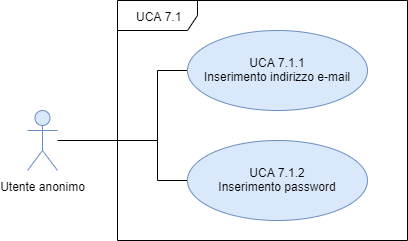
\includegraphics[scale=0.5]{sezioni/UseCase/Immagini/UCA7.1.png}
\end{figure}
\subsection{UCA 7.1 - Ordinamento della lista degli accessi presso un’organizzazione}%sea level
\begin{itemize}
\item \textbf{Attori primari:} Utente anonimo;
\item \textbf{Precondizione:} L’utente ha a disposizione una lista di accessi presso uno o più luoghi di un'organizzazione;
\item \textbf{Postcondizione:} l’utente ottiene una lista di accessi presso i luoghi dell’organizzazione selezionata nell’ordine richiesto;
\item \textbf{Scenario principale:} L’utente seleziona la funzionalià “Ordinamento” che preferisce fra le disponibili
	\begin{itemize}
	\item UCA 7.2.1 Ordinamento per data (da più recente a meno recente) della lista degli accessi presso un’organizzazione;
	\item UCA 7.2.2 Ordinamento per data (da meno recente a più recente) della lista degli accessi presso un’organizzazione.
	\end{itemize}
\end{itemize}

\subsubsection{UCA 7.1.1 - Ordinamento per data (da meno recente a più recente) della lista degli accessi presso un’organizzazione}%fish level
\begin{itemize}
\item \textbf{Attori primari:} Utente anonimo;
\item \textbf{Precondizione:} L’utente ha a disposizione una lista di accessi presso uno o più luoghi di un organizzazione;
\item \textbf{Postcondizione:} L’utente ottiene una lista di accessi presso i luoghi; dell’organizzazione selezionata in ordine per data (dalla più recente alla meno recente).
\end{itemize}

\subsubsection{UCA 7.1.2 - Ordinamento per data (da meno recente a più recente) della lista degli accessi presso un’organizzazione}%fish level
\begin{itemize}
	\item \textbf{Attori primari:} Utente anonimo;
	\item \textbf{Precondizione:} L’utente ha a disposizione una lista di accessi presso uno o più luoghi di un organizzazione;	
	\item \textbf{Postcondizione:} L’utente ottiene una lista di accessi presso i luoghi dell’organizzazione selezionata in ordine per data (dalla meno recente alla più recente).	
\end{itemize}

\subsection{UCA 7.2 - Filtro per luogo della lista degli accessi presso un’organizzazione}%sea level
\begin{itemize}
	\item \textbf{Attori primari:} Utente anonimo;
	\item \textbf{Precondizione:} L’utente ha a disposizione una lista di accessi presso uno o più luoghi di un'organizzazione;
	\item \textbf{Postcondizione:} L’utente ottiene una lista di accessi presso un singolo luogo selezionato (che può coincidere con la lista di partenza se l’organizzazione ha un singolo luogo a disposizione)	
	\item \textbf{Scenario principale:}
	\begin{itemize}
		\item L’utente seleziona la funzionalità “Filtro per luogo”;
		\item L’utente seleziona un luogo dell’organizzazione.
	\end{itemize}
\end{itemize}